%deixar chapter vazio - exatamente como está. Preencher o documento apenaas apartir de section.
\chapter*[]{}

\section{Tema}

A ABNT indica a elaboração de uma lista de ilustrações com todos os itens arrolados e designados por seu nome específico, conforme a ordem que aparecem no texto (Figura 1, Fotografia 1, Gráfico 1, Quadro 1, entre outros). Também recomenda, quando necessário, a elaboração de lista própria para cada tipo de ilustração. No entanto, não determina um número mínimo de ilustrações para tal lista específica.

\subsection{Delimitação do tema}
Aqui vai a delimitação do tema se tiver


\index{elementos textuais}A norma ABNT NBR 15287:2011, p. 5, apresenta a
seguinte orientação quanto aos elementos textuais:

\begin{citacao}
	O texto deve ser constituído de uma parte introdutória, na qual devem ser
	expostos o tema do projeto, o problema a ser abordado, a(s) hipótese(s),
	quando couber(em), bem como o(s) objetivo(s) a ser(em) atingido(s) e a(s)
	justificativa(s). É necessário que sejam indicados o referencial teórico que
	o embasa, a metodologia a ser utilizada, assim como os recursos e o cronograma
	necessários à sua consecução.
\end{citacao}

Consulte as demais normas da série ``Informação e documentação'' da ABNT
para outras informações. Uma lista com as principais normas dessa série, todas
observadas pelo \abnTeX, é apresentada em \citeonline{abntex2classe}.

\section{Problema}
escreva aqui...


\section{Objetivos}
escreva aqui...

\subsection{Objetivo Geral}
escreva aqui...

\subsection{Objetivos Específicos}
\begin{enumerate}
	\item objetivo especifico aqui...
	\item objetivo especifico aqui...
\end{enumerate}

\section{Justificativa}
escreva aqui...\\

\section{Referencial Teórico}
Este parágrafo serve apenas para explicar as citações de referências. Esta próxima linha mostra uma citação indireta. Conforme~\citeauthoronline{bourg2013physics}, o quadrado não é redondo e o círculo não é quadrado. Esta próxima citação é do tipo direta, onde copiamos uma frase inteira do autor. Poderíamos refletir sobre a "existência de quadrados redondos e circulos quadrados"~\cite{ericson2004real}. Seria uma reflexão válida?.

Este parágrafo serve apenas para explicar como é inserido uma imagem. A figura precisa sempre ser referenciada no texto da seguinte forma: A Figura~\ref{fig:figura1} apresenta uma representação gráfica de uma esfera a esquerda, e um cubo a direita. No campo caption vai uma label (que é unica em todo texto e pode ser referenciada em qualquer lugar do texto). No campo legend, vai da onde a figura saiu ... se for de um livro precisa fazer a refrencia...

\begin{figure}[htb]
	\caption{\label{fig:figura1} Legenda da figura}
	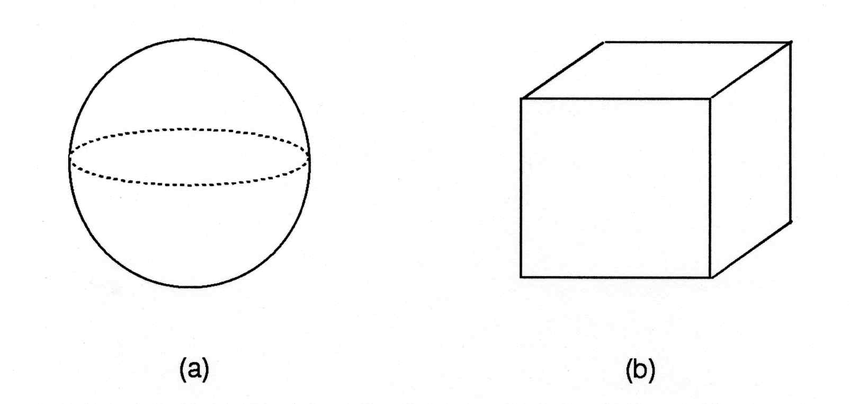
\includegraphics[width=\textwidth]{figuras/figura1.png}
	\legend{Fonte: \cite{bourg2013physics}. }
	
\end{figure}


Aqui nesse parágrafo um trecho de código em C++. O Algoritmo~\ref{lst:codigo1} apresenta um trecho de código mágico.

\begin{lstlisting}[caption={Exemplo de laço},label={lst:codigo1}]
	void func(int){
	for(int =0;i<10;i++){
		fprintf("asdfas fddfsadf");
	
		}
	}
\end{lstlisting}



\section{Metodologia}
escreva aqui...

\subsection{Cronograma}
escreva aqui...

